% ------------------------------------------------------------------------ %
% !TEX encoding = UTF-8 Unicode
% !TEX TS-program = pdflatex
% !TEX root = ../Tesi.tex
% !TEX spellcheck = it-IT
% ------------------------------------------------------------------------ %
%
% ------------------------------------------------------------------------ %
% 	Problem analysis and proposed solution
% ------------------------------------------------------------------------ %
%
\chapter{Problem Analysis}
%
\label{cap:probanalysis}
%
% ------------------------------------------------------------------------ %
%

In this chapter the specific problems of this work will be detailed and analyzed, explaining what are the limits and the constraints the challenge has. The chapter starts with a brief recap, followed by the proper definition of what I faced, while in the last part there is a list of constraints my architecture will have fulfilled in order to have a universal and functional solution.
  

\section{Brief recap} \label{facedProblem}
In the previous chapter, number \ref{cap:statoarte}, I have defined IoT and WoT, pointing out the main differences between the two definitions. In particular I focused on the problem of the interconnection between the two different paradigms. 
The IoT can be seen as a network, in which not only standard computers are connected as nodes, but also smart objects: they are "first class citizens" of the internet, they have a connectivity module, they have the capacity to "talk" each other. But, due to some constraints, in particular power consumption constraints, it is not possible to consider the IoT as a big unified network, because devices have different communication protocols and not all of them are compatible with each other to offer communication. The result is a non standardized confused cloud of protocols, systems and technical stacks. Solutions are often proprietary and closed, even if some open solutions exist.\\
The WoT is the election of the smart objects to "first citizens" of the web, the web has a fundamental role as unifying layer, it is standardized, it easily reachable by everyone and there is no need of particular requirements on devices. The idea is bringing the devices to the web. The fundamental requirement is the implementation of TCP/IP and HTTP protocols. Not every object has the capacity to provide this connection, but most of them could, also with the help of a gateway which can be also called \textit{reverse proxy}. In this chapter I am considering only devices that have this feature.\\
After this brief recap of what has been said about the Internet of Things and the Web of Things in the state of the art chapter, here I am trying to define with more precision the problem I am going to face: which its constraints and its possible goals are.

\section{Definition} \label{problemdefinition}
As anticipated above, I am going to take into account only devices that can be somehow connected to the internet, the ones which provides an implementation of HTTP protocol in particular, while in the substrates the stack can be left "opened": each vendor can implement its solution only if it provides a classical connection on the top. This statement can be seen as a  "little relaxation" of the constraints previously announced.\\
Having done this clarification, now I am defining the problem. \\
As said the Web of Things is the "unification" layer built on top of Internet of Things, it does not replace IoT, it is a completion. There is a sort of vertical hierarchy. If both must coexist a sort of communication between them is fundamental to assure the right functioning of the entire stack. We have clear in mind what can be considered WoT for the final user: a sort of control center, reachable by a web browser, where anyone can control the smart objects he has rights on. Also what is IoT for final users is clear: it is a heterogenous world, a world made of objects they can control through smartphone, for instance. So we have an idea of the two parts we have to connect: on one side the well known web paradigm, with its programming languages, its limited number of web browsers; on the other a myriad of objects that have in common the possibility to act as web servers, managed through HTTP calls. \textit{How can we let these two parts talk?} This is the question that my thesis is trying to answer. My work is a concrete solution, it is about creating or refining some communication methods.\\
So I am trying to let different worlds talk using  well known tools: I have just said I am putting IoT and WoT in communication, but with the warranty that the smart objects can behave as web servers. So I am defining a method to connect different, "vertical" worlds, put one on the top of the other using a "horizontal" system: devices have HTTP endpoints that elect them to citizens of the web. But this does not guarantee they have a right behavior to be integrated in a heterogeneous and user friendly application. The result is a vertical connection that covers all the protocol stack, from the physical layer to the application one, while the last part of the connection is a "double step connection", a hardware part that guarantees the online presence of the device, and a software part that assure the right behavior and the standardization of the communication. Figure \vref{3.1:problemdef}, describes what has just been explained: the green arrow indicates what is seen externally, the protocol stack, it links directly the application layer with the underlying ones. The red arrows indicate what I am proposing in this thesis: red one in the layer 4 is our requirement, the fact that the smart objects can act as web servers that are components of layer 7. The second red arrow, the one included in the application layer is the representation of what my work is trying to achieve, the software component of the full integration, as above described. As said the red arrow is all in the application layer, it remains "horizontal" in respect to the stack, it can be seen as an HTTP call done from the client, put in the "cloud" (note that what here is considered client can be the backend, the server, of a third-party application). The double side of the arrows stands, obviously, for the possibility to enable communication both sides, packing and unpacking information.

\begin{figure}[h]
	\centering
	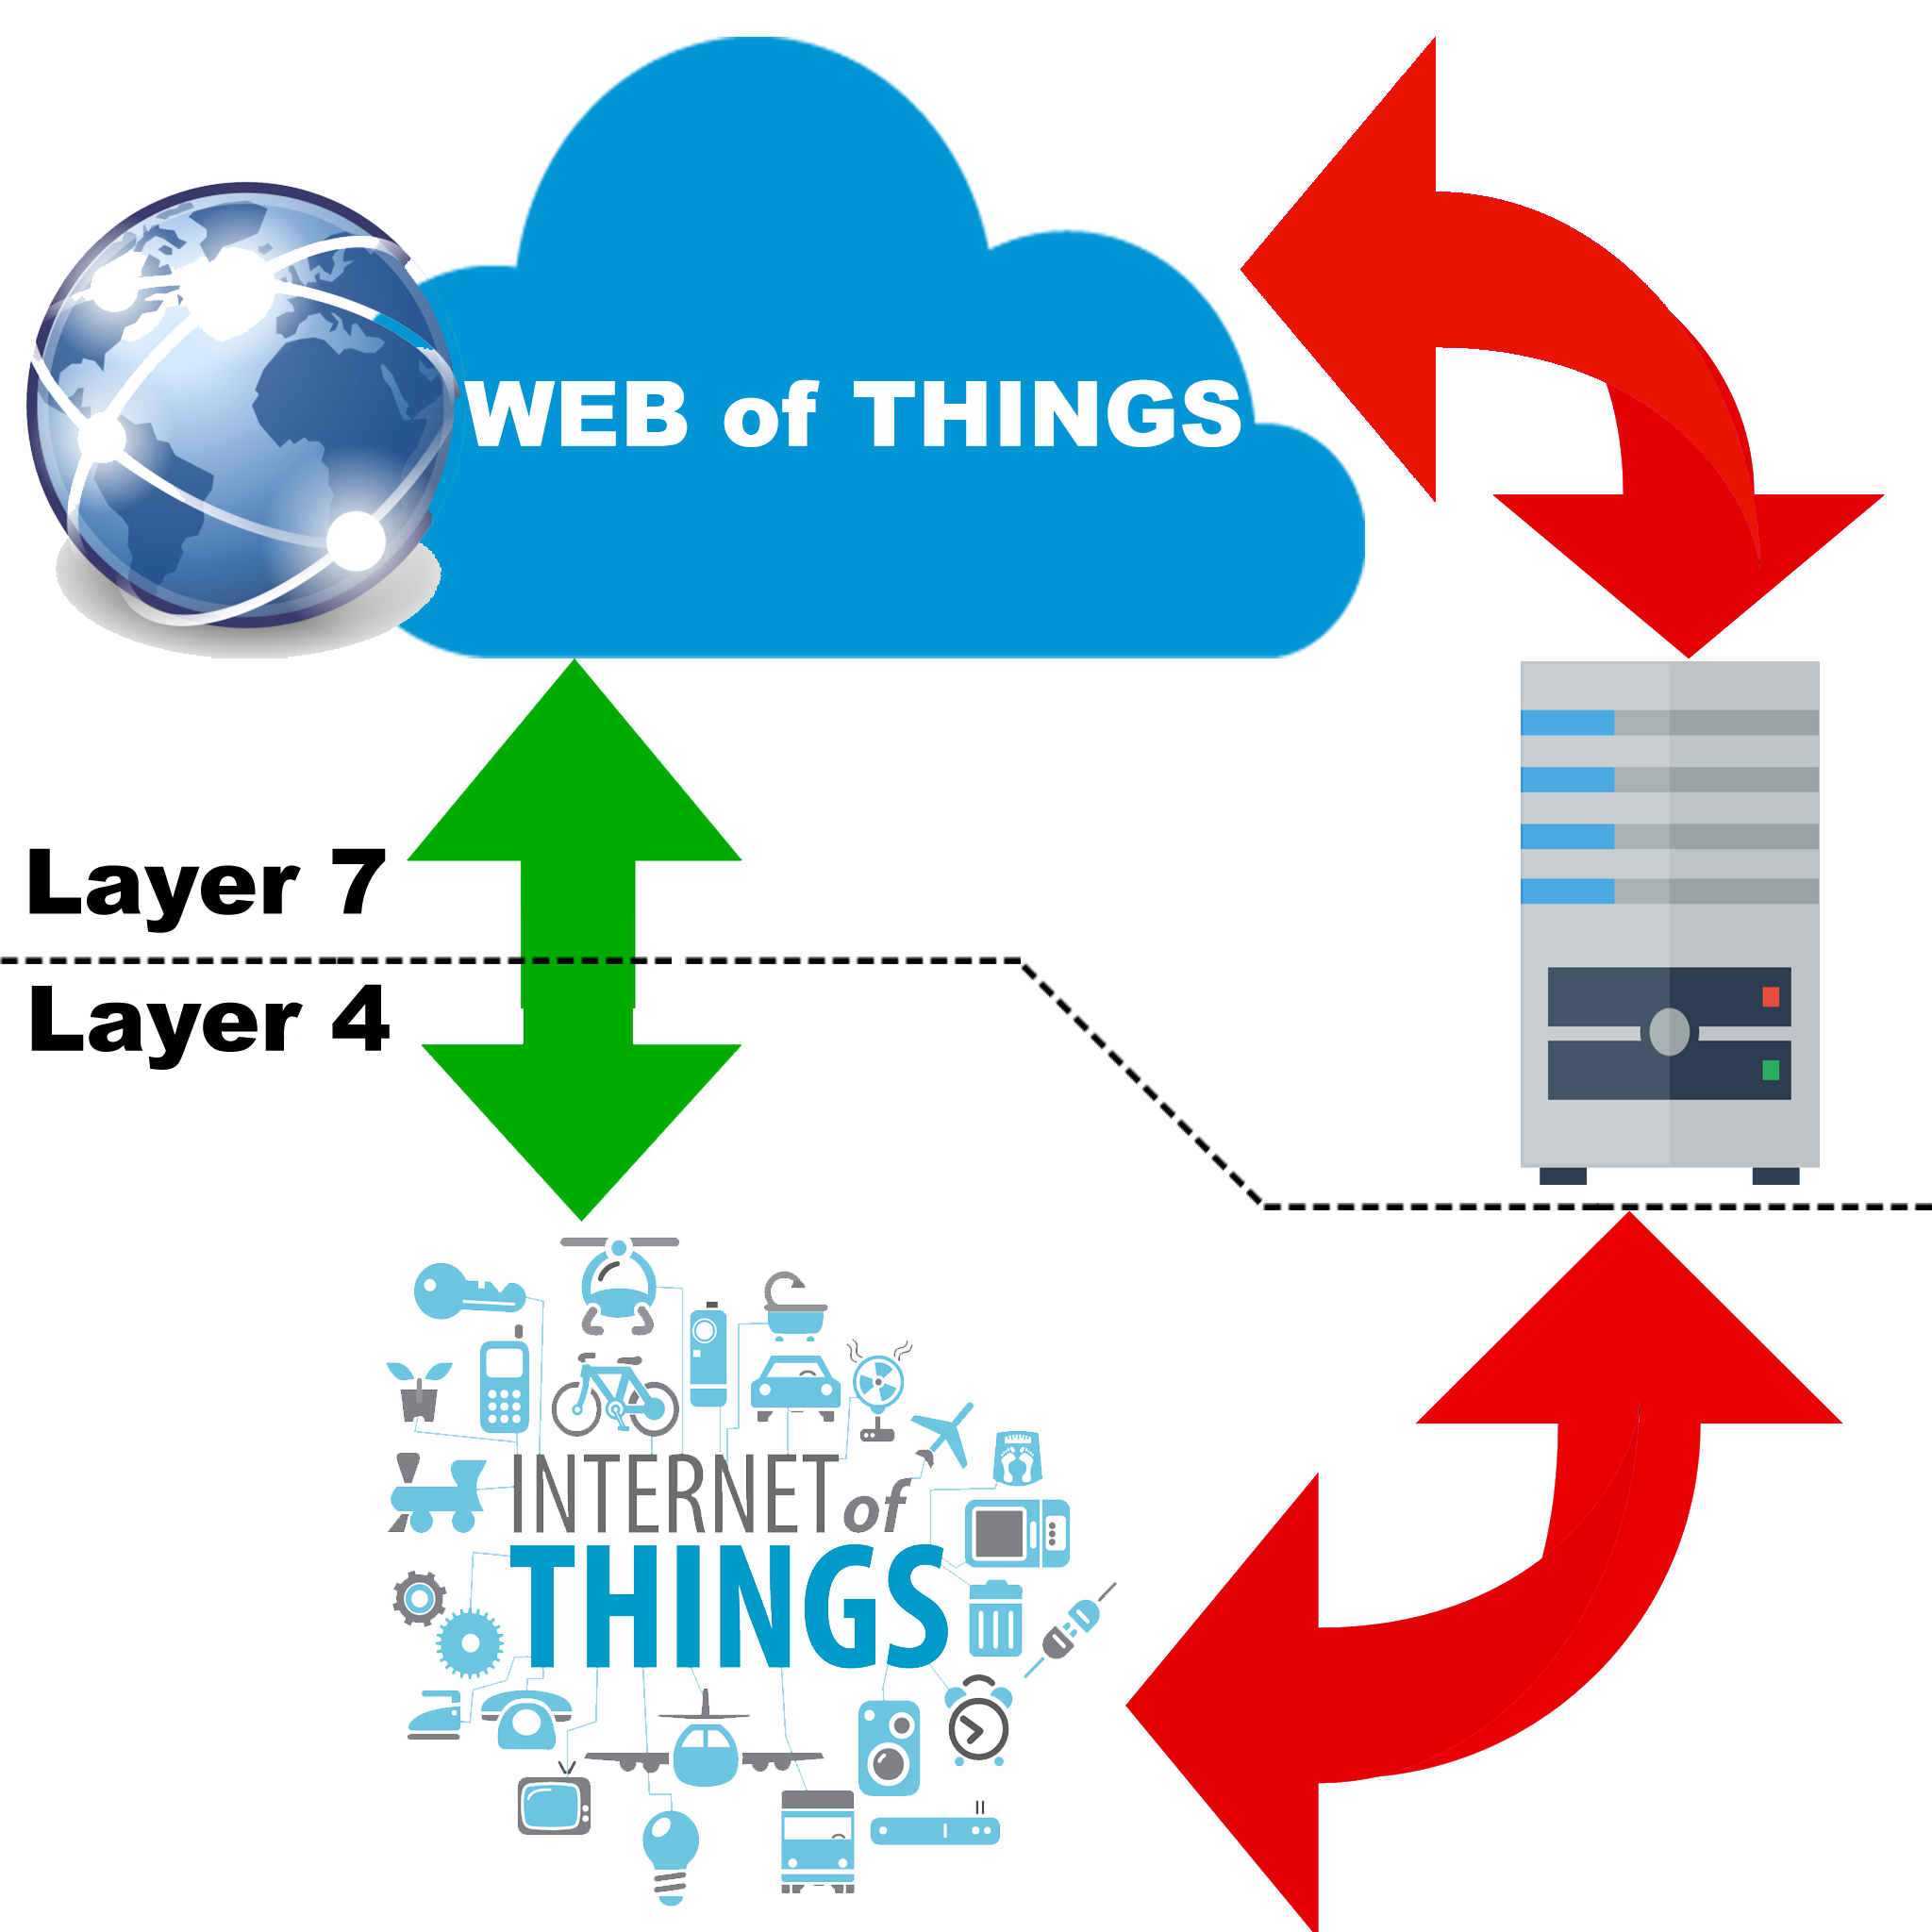
\includegraphics[width=.8\textwidth]{problemdef}
	\caption{Stack result vs double step implementation}
	\label{3.1:problemdef}
\end{figure}

The important point is having a message with a well defined content: it is what the two parts must write and read, so it has to be clear for machines, must be compliant with all the requests of \textit{M2M (Machine-to-Machine) communication}. On the other hand, a developer must be capable of reading and understanding what is going on in order to debug to solve errors or to write a customizable user application, so the communication must require also to match the \textit{M2H (Machine-to-Human) communication} and \textit{H2M (Human-to-Machine) communication} requirements. These types of communications are some constraints of my work and are explained in the next section \ref{problemconstraints}. \\
So the problem I am going to face is the \textit{lack of a standard communication method} between the smart objects and the web interfaces already present. What I am going to define in this thesis is a new "communication", efficient and practical. This can be seen as two distinct parts of the development: the choice of the "container" and the proper definition of the syntax. As said above, types of communications are a sort of constraints for the defined syntax, but also the choice of the "container" is not completely free, it has to match some fundamental constraints to assure the correct HTTP transmission of a message or a file. \\
Next sections will properly define all the constraints of the given problem and propose a solution that fulfills them all.

\section{Constraints} \label{problemconstraints}
In this section I would like to list a set of  constraints for the defined problem, that become requirements that the solution must meet. The section should be divided into two parts, the first for the requirements of the container, the second for the ones of the syntax, but the two sections are closely related so here I preferred to keep the two parts united, indicating wherever possible which of the part that particular constraint acts on.\\
Here is the list:

\begin{itemize}
	\item \textit{M2M communication:} M2M communication is defined as a communication in which the two interlocutors are not humans. It is a communication completely handled by machines and computers \cite{cha2009trust}. It can be considered one of the fundamental enabling technologies of the Internet of Things, it permits object to communicate without humans being involved. This type of communication has to be stricter respect to M2H: the subject reading the content is a computer, it has no a semantic idea of what is written, it can, at most, understand the syntax. So a clear, defined syntax with a well fixed structure  must be set in order to make everything understandable to a computer. Obviously the machine has also to able to write the code or the file that will be sent. Anyway, the problem of what is understandable for a machine is a common "problem" to all fields in computer science and engineering.
	
	\item \textit{M2H/H2M communication:} I grouped these two constraints because they are similar, they include some similar behaviors, in fact somehow the solution I am writing has to reach at least a human being, the owner of the smart space. In order to check what is going on and control the behavior of smart devices the user must understand what he sees on a web application. This constraint can be considered "indirect" for my work: it must be somehow adapted to a UI, the one of a control center application developed on top of the file I will provide. So it means that my work does not reach the user directly but it means that it should be possible to translate it easily into something the user can understand without too much effort. That means I have to use variables and values in a univocal way, in order to permit the web app a clean and meaningful translation. These considerations are valid for M2H communication. Regarding H2M communication the user must be able to easily impart commands and the inverse procedure of translation needs to be as simple as possible. So the user has some constraints: he cannot use free natural language, the problem is still the same, computers are not able to semantically understand natural language. 
	
	\item \textit{Easy readable:} What I am going to define is a sort of description of a smart space that must be readable by machines and by humans, as explained above. This does not imply the easy readable property: a thing can be read by human or machine but with difficulty. The desired property here is the fact that both humans and machines will be able to read the content of the smart space without much effort. This streamlines all the procedures. A machine that has to execute a command or retrieve information has to do it very quickly, if something must be notified to the user, the content to (write and) read must not be an obstacle, in terms of speed or resources spent to assure the right communication. For humans, we can distinguish two categories, developers and users. For users the situation can be mitigated by the presence of a web application between my work and what he sees on the web pages. I will provide a description of objects which will be embedded into third-party applications. In this way the user does not see directly what I have done: developers are the people who use data provided by my system to construct a web application. Two are the main reasons they need understandable data, developers need data to be easy readable in order to easily integrate them in applications and also to debug the system. The error can be in the written code, but the source remains my work, having it clear in mind, it can help to quickly debug.
	
	\item \textit{Reconfigurable:} we are talking about smart spaces, composed of smart objects, they are usually relatively small and so they can be moved easily (some of them, though may be bigger, such as industrial machinery). Another issue can be the fact that, being powered by batteries, objects can turn off due to low level battery status. These two just explained situations appear to my system as a change of of the smart space: it is necessary to reconfigure it, in order to output the current situation without having "dead devices" or moved ones into the described space. Moving a device, we can have the situation where a sensor, for example, is moved from a room to another, so the total number of devices is not changed but the configuration is. My system must be able to detect the "loss" of one of them in some place and the "gain" of the same one in another. 
	
	\item \textit{Fast:} being fast is one of the essential constraints of my work. I have just stated that the reconfigurable property is desired, to handle the change of the spaces my thesis is going to describe. But how fast my system reconfigures all the list of objects becomes fundamental. No latency is permitted. Think about an alarm or a thermometer which goes out due to the level of the battery: the user must be notified and aware as soon as possible. The user cannot be kept without any protection for his home or without heating in winter. There should be a mechanism, a sort of listener, that understands when something is changed and reports quickly to the third-party application the user uses.
	
	\item \textit{Lightweight:} Another constraint to our system is the fact that whatever system I choose to be the solution it must be lightweight. This is needed because it goes on the web, the third-party application server requires information from the objects that it collects, packs it and sends to the user. The user can see its configuration through a web browser that, as a client, downloads the required page. If we want information to be notified quickly, information should necessarily  be lightweight. So my solution has to take into account the fact we are talking of the Web of Things, and the word "web" implies some constraints by definition: the one we are interested in here is the latency and the transmission time, due to the physical limits of the cable or the materials that constitute the network infrastructure. 
	
	\item \textit{Modular:} the language or type of file chosen must be modular. The faced problem is modular itself: it is necessary to group lots of IoT devices into one singular description. It must be a description of the smart space: it is composed, for instance, of rooms. And also in each room there can be a hierarchy of devices, in addition the objects with a gateway need to be described as coupled, and only one gateway can have multiple devices to control. So the solution also has to be modular, it must be possible to write different configurations. It is necessary to define some building blocks, that can be placed almost everywhere in the hierarchy. The length or the number of levels that can be nested should be variable, each smart space has different particularities: starting from a city to a living room. My solution must be universal: a thermometer, for instance, can be put in both of the listed places without specifying where it is and without changing internally its properties due to the position.
		
	\item \textit{Complete:} the chosen solution must be complete, in the sense that it must be able to write down every configuration. It should be possible to describe any kind of object, it has to own each kind of smart object present on the market, with their properties, status and commands. It should also be possible to insert each object in the hierarchy almost everywhere, even if, obviously, some rules are needed to assure the right syntax and the right structure. A "language" that is not complete cannot be accepted, it must be able to describe any given smart place, my solution tries to be a unifying method for developers that can count on it as a consistent description of the space, the "source" of what they have to output to the user.
	
	\item \textit{Extensible:} the solution must be extensible, because every day new objects become smart. With the technical innovation it will be possible to increasingly miniaturize the chips needed to offer a connection, to become smart. My language needs to be extensible, when a new sort of product comes on the market my language has to define a standard for it, according to the object's properties, states and features. It must be always possible to do that, there should not be limits to the number of building blocks my solution is going to define, because we do not know today where the "smartness" of objects is going to go, we do not know the level of miniaturization and power saving that will be reached in the future. Being extensible means being a valid alternative also in the future, writing a solution that only fits "today" objects without the possibility to expand limits my work to be just a "photograph" of the current state. With the growth of the number and types of smart devices, the extensible property becomes fundamental to obtain another property: completeness.
	
\end{itemize}
 
The listed requirements, as already told in some of them, are, sometimes, general, in the sense that they have to be respected for the final product: a global and complete structure that starts from the smart object and arrives to the user's web browser. This is because the problem I am facing is very big and complex, and it is transversal to the existing technologies, so the whole system must work properly. Keeping in mind what I have just stated, some of these constraints become fundamental requirements that my system must meet, some others, for instance the M2H communication, are only indirect or partial requirements: my work has to be clear for the developer, who knows what variables are, how a file can be accessed, parsed and processed but it can be less clear to an average user who wants, out of curiosity, see what is under the hood.

\bigskip
\bigskip
\bigskip

In the next chapter I am presenting my idea, the so called solution to the given problem, explaining what I have done, my considerations about the situation here faced. I am defining both the container and the syntax, or better the structure, of my work; these two parts are the fundamental ideas that are the bases to construct my thesis. 


%
% -----------------------------END------------------------------------- %